\documentclass[tikz]{standalone}

\usepackage[T1]{fontenc}
\usepackage[english]{babel}

\usepackage{standalone}

\usepackage{pgfplots}

\usetikzlibrary{calc, 3d}

\begin{document}
    \begin{tikzpicture}
    	\node (fos) {
            \includestandalone[mode=buildmissing, height=1.5cm]{figures/errors/facet/fos}
        };
        \path (fos.west) node[anchor=east] (fib) {
            \includestandalone[mode=buildmissing, height=1.5cm]{figures/errors/facet/fib}
        };
        \path (fib.west) node[anchor=east] (bos) {
            \includestandalone[mode=buildmissing, height=1.5cm]{figures/errors/building/bos}
        };
        \path (fos.east) node[anchor=west] (fig) {
            \includestandalone[mode=buildmissing, height=1.5cm]{figures/errors/facet/fig}
        };
        \path (fig.east) node[anchor=west] (bos) {
            \includestandalone[mode=buildmissing, height=1.5cm]{figures/errors/facet/fus}
        };
    \end{tikzpicture}
\end{document}
